\documentclass{standalone}
\usepackage{tikz}
\begin{document}
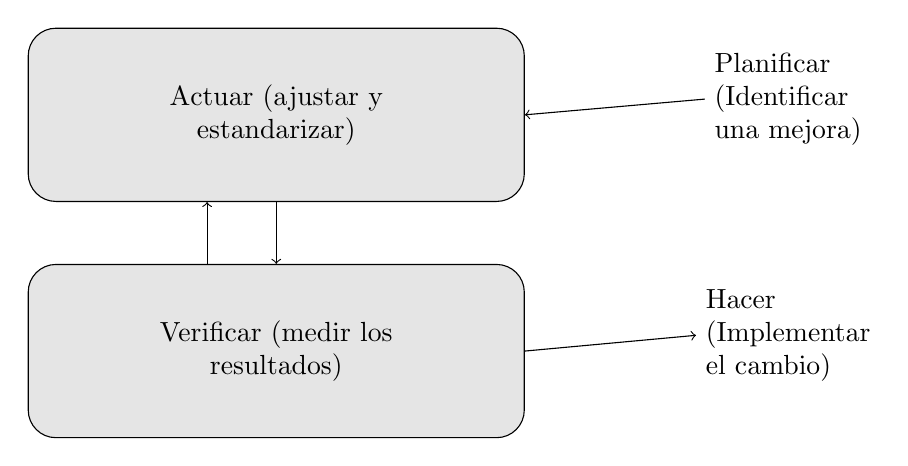
\begin{tikzpicture}
    % Nodos principales alineados manualmente
    \node[draw, fill=gray!20, rounded corners=10pt, minimum width=6.3cm, minimum height=2.2cm, align=center] (actuar) 
        at (0,0) {Actuar (ajustar y\\ estandarizar)};
    \node[draw, fill=gray!20, rounded corners=10pt, minimum width=6.3cm, minimum height=2.2cm, align=center] (verificar) 
        at (0,-3) {Verificar (medir los\\ resultados)};
        
    % textos externos alineados manualmente
    \node[align=left] (planificar) at (6.5,0.2) {Planificar\\ (Identificar\\ una mejora)};
    \node[align=left] (hacer) at (6.5,-2.8) {Hacer\\ (Implementar\\ el cambio)};
    
    % Flecha principal: Actuar -> Verificar
    \draw[->] (actuar.south) -- (verificar.north);

    % Flecha secundaria, desplazada a la izquierda: Verificar -> Actuar
    \draw[->] ([xshift=-25pt]verificar.north) -- ([xshift=-25pt]actuar.south);

    % Flechas rectas para textos externos
    \draw[->] (planificar.west) -- (actuar.east);
    \draw[->] (verificar.east) -- (hacer.west);
\end{tikzpicture}
\end{document}
